\documentclass[coda.tex]{subfiles}
\begin{document}

\section{Inferring Local Factorization}\label{sec:inferring_local_factorization}
Here we present several approaches to inferring the local factorization of subspaces, a crucial subroutine of CoDA.
We note that in many cases where domain knowledge is available, simple heuristics may suffice, e.g. in our Goal-conditioned RL experiments discussed in Section \ref{sec:experiments} where a simple distance-based indicator function in the state space was used. 
However, as such heuristics may not be universally available, the question of whether data-driven approaches can successfully infer local factorization is of general interest.
We note that the performance of CoDA will improve alongside future improvements in this inference task (motivating future work in this area), and that inferring the local factorization in general is an easier task than learning the environment dynamics.

We begin by presenting two methods for inferring local factorization, derived from variants of a next-state prediction task, which we here refer to as SANDy for Sparse Attention Neural Dynamics.
To verify the merits of SANDy in the local factorization inference task, we evaluate two SANDy variants in controlled settings where the ground truth factorization is known: first in a synthetic Markov process (MDP without actions), and second in Spriteworld.
This label information is used only to evaluate performance, and not to train the SANDy parameters.
The SANDy-Transformer model was used for the Online RL experiments presented in Section \ref{sec:experiments}.

\subsection{Methods}\label{subsection_learning_factorization}

We propose two Sparse Attention for Neural Dynamics (SANDy) models. In each case we seek to learn a function (or mask) $M(s, a) \to \{0, 1\}^{(|S|+|A|)\times|S|}$ whose output represents the adjacency matrix of the local causal graph, conditioned on the state and action. We note that $M(s, a)_{i,j} = 0$ alone is insufficient, in general, to determine the local subspace $\L \subset \S \times \A$, since there may be multiple disconnected subspaces $\L_k$ with $M_k(s, a)_{i,j} = 0$ whose union $\bigcup_k \L_k$ has $M_{\cup k}(s, a)_{i,j} = 1$. This can be resolved by our Proposition \ref{proposition_union_of_local_sets} if we also force the relevant structural equations to be the same. For now, we assume the mask determines the local subspace, and leave exploration of this possibility to future work. Empirically, we will see that our assumption is reasonable.

\paragraph{SANDy-Mixture} 

The first model is a mixture-of-MLPs model with an attention mechanism that is computed from the current state.
Each component of the mixture is a neural dynamics model with sparse local dependencies. 
For a given component, the key idea is to train a neural dynamics model to predict the next state $h(s_t, a_t) \approx s_{t+1}$ and approximate the masking function by thresholding the (transpose of the) network Jacobian of $h$, $[\mathbf{J}(s, a)]_{i, j} = \frac{\delta}{\delta [s, a]_j} [h(s, a)]_i$. Intuitively, we can think of $\mathbf{J}$ as providing the first-order element-wise dependencies between the predicted next state and the network input. We then derive the local factorization by thresholding the absolute Jacobian 
\begin{equation}
M_\tau(s, a) = \indicator{|\mathbf{J}(s, a)| > \tau},    
\label{eq:thresh}
\end{equation}
where $\indicator{\cdot}$ represents the indicator function and $\tau$ is a threshold hyperparameter.

To estimate the network Jacobian, we note that for standard activation functions (sigmoid, tanh, relu), it can be bound from above by the matrix product of its weight matrices. To see this, let $h_\theta$ be an $L$-layer MLP parameterized by $\theta = (\W^{(1)}, \B^{(1)}, \cdots, \W^{(L)}, \B^{(L)})$ with activation $\sigma$ with bounded derivative $\sigma'(x) \leq 1$, and note that for each layer $\bm{h}^{(\ell)} = \sigma(\W^{(\ell)}\bm{h}^{(\ell -1)} + \B^{(\ell)})$ we have:
\begin{align*}
	\Bigg\vert\frac{d\bm{h}^{(\ell)}_j}{d\bm{h}^{(\ell-1)}_i}\Bigg\vert &\leq \Big\vert\W^{(\ell)}_{ji}\Big\vert.
\end{align*}
Then, using the chain rule, triangle inequality, and the identity $|ab| = |a||b|$, we can compute:
\begin{align*}
	\Bigg\vert\frac{d\bm{h}^{(\ell)}_j}{d\bm{h}^{(\ell-2)}_i}\Bigg\vert &\leq \Bigg\vert\frac{d}{d\bm{h}^{(\ell-2)}_i}   \W^{(\ell)}_{j\cdot} \bm{h}^{(\ell-1)}\Bigg\vert =\Bigg\vert\W^{(\ell)}_{j\cdot} \cdot \frac{d\bm{h}^{(\ell-1)}}{d\bm{h}^{(\ell-2)}_i} \Bigg\vert \\
	&
	\leq \sum_k \Bigg\vert\W^{(\ell)}_{jk} \frac{d\bm{h}^{(\ell-1)}_k}{d\bm{h}^{(\ell-2)}_i} \Bigg\vert 
	\leq \Big\vert\W^{(\ell)}_{j\cdot} \Big\vert \cdot \Big\vert\W^{(\ell-1)}_{\cdot i} \Big\vert.
\end{align*}
Expanding this out to multiple layers, we see that $\big\vert \mathbf{J}_\theta(s, a)\big\vert  \leq \prod_{\ell \in [L]} |\W^{(\ell)}|$, as desired. We use this upper bound to approximate the network Jacobian of an MLP by setting $\mathbf{\hat J} = \prod_{\ell \in [L]} |\W^{(\ell)}|$. A similar idea is used by \cite{germain2015made,lachapelle2019gradient}, among others, to control element-wise input-output dependencies.

We use this static approximation $\mathbf{\hat J}$ to facilitate learning a sparse dynamic mask by specifying a mixture model $h(s, a) = \sum_i \alpha^{(i)}_\phi(s,a) h^{(i)}_\theta(s,a)$ over the environment dynamics (with $\sum_i \alpha^{(i)}_\phi(s,a) = 1 \ \forall \ (s, a)$), where each component $h^{(i)}_\theta$ is an MLP as specified above with a sparsity prior on its Jacobian bound $\mathbf{\hat J}^{(i)}$ to encourage sparse (i.e. well-factorized) local solutions. The dynamic mask is computed by first approximating the Jacobian, $\mathbf{\hat J}(s,a) = \sum_i \alpha^{(i)}_\phi(s,a)\mathbf{\hat J}^{(i)}$, then thresholding by $\tau$ as in Equation \ref{eq:thresh}.

Note that we assume the mixture components $\alpha$ are a function of the current state and action alone; in other words the factorization (captured by the network Jacobian of each component) can be \emph{locally inferred}.
The next-state prediction is given by $\hat \s_{t+1} = ( h_\theta^{(1)}(\s_t, \mathbf{a}_t), \cdots, h_\theta^{(N)}(\s_t, \mathbf{a}_t))^T \bm{\alpha}_\phi(\s_t, \mathbf{a}_t)$. To train the model, we optimize the objective:
\begin{equation}\label{eq:mixture-mlp}\small
\underset{\theta, \phi}{\minimize} \ 
  \frac{1}{|\mathcal{D}|} \Big( \sum_{(\s_t, \mathbf{a}_t \s_{t+1}) \in \mathcal{D}} ||\s_{t+1} - h(\s_t, \mathbf{a}_t)||_2^2 \Big) 
  + \lambda_1 S(\theta) +  \lambda_2 R(\phi) + \lambda_3 ||(\theta, \phi)||_2
\end{equation}
where $S(\theta) = \frac{1}{K} \sum_i |\hat{\mathbf{J}}_\theta^{(i)}|_1$ puts an $\ell_1$ prior on each mixture component to induce sparsity,
and $R(\phi)$ encourages high entropy in the attention probabilities
\[
  R(\phi) = \frac{1}{|\mathcal{D}|} \sum_{\s \in \mathcal{D}} \sqrt{\frac{1}{N}\sum_{j \in [N]} [A_\phi(\s, \mathbf{a})]_j}.
\]



We note that more sophisticated methods of computing Jacobians of neural networks--including architectural changes and optimization strategies \cite{arjovsky2017wasserstein}---have been proposed, and could in principle be used here as well.

\paragraph{SANDy-Transformer}

As an alternative model, we use a transformer-like architecture that applies self-attention between a set of (potentially multi-dimensional) inputs \cite{vaswani2017attention, lee2018set}. Our architecture is composed of a stacked self-attention blocks. Each block accepts a set of inputs $X = \{x_i \in \R^n\}$ and composes three functions of each input: query $Q: \R^n \to \mathbb{R}^d$, key $K: \R^n \to \mathbb{R}^d$, and value $V: \R^n \to \mathbb{R}^m$. The block returns a set of outputs $\{y_i \in \mathbb{R}^m\}$ of size $|X|$, each of which is computed as: $y_i = A_i^TV(X)$, where $A_i = \textrm{softmax}\big(\sum_j(Q(x_i)_j K(x_j)_i)\big)$ (note that $V(X)$ is a matrix of size $|X| \times m$). We approximate the block mask (approximate Jacobian) as $A = [A_1, A_2, \dots, A_{|X|}] \in \R^{|X| \times |X|}$, and the full network mask as the product of the block masks (as in the SANDy-Mixture). We used two-layer MLPs for each function $K, Q, V$ in Spriteworld and three-layer MLPs in Pong. 

To apply this architecture to our problem, we first embed each state and action component (single feature, or group of features) into $\R^n$ to produce a set of inputs $X$ and pass this through each stacked self-attention block to obtain a set of outputs $Y$. We then discard any output components that correspond to the action features to obtain the next state prediction and mask. The network $h$ is trained to minimize mean squared error:
\begin{equation}\label{eq:sandy-transformer}\small
\underset{\theta}{\minimize} \ 
  \frac{1}{|\mathcal{D}|}\sum_{(\s_t, \mathbf{a}_t \s_{t+1}) \in \mathcal{D}} ||\s_{t+1} - h(\s_t, \mathbf{a}_t)||_2^2.
\end{equation}
Unlike the SANDy-Mixture, no sparsity regularizers are applied, as we found the sparsity induced by the softmax attention mechanism to be sufficient. 

\subsection{Evaluation environments}

\paragraph{Synthetic Markov Processes}
We investigate the capacity of the SANDy-Mixture to learn simple factorized transition dynamics under a globally factored Markov Process (\textsc{StationaryMP}).
Unlike the general MDP setting, no agent/policy is considered.
However the ability to train an unconstrained dynamics model to approximate factorized environment dynamics is an important subtask within our overall approach.
Assuming a spherical Gaussian prior over the initial states $\s^0 \in \R^9$, the \textsc{StationaryMP} is entirely specified by transition distribution $p(\s^{t+1}|\s^t)$.
We assume that the state transitions factorize (globally) into three parts.
Denoting by $\s_{n \cdots m}^t$ the $n$-th through $m$-th dimensions of the time $t$ state $\s^t$, we have:
\[
p(\s^{t+1}_{1\cdots9} | \s^{t}_{1\cdots9}) =
  p(\s^{t+1}_{1\cdots4} | \s^{t}_{1\cdots4})
  p(\s^{t+1}_{5\cdots7} | \s^{t}_{5\cdots7})
  p(\s^{t+1}_{8,9} | \s^{t}_{8,9}).
\]
In other words, we have a block-diagonal transition matrix comprising three blocks with sizes $4$, $3$, and $2$, respectively.
In our case, all transition factors are deterministic non-linear mappings, e.g. $p(\s^{t+1}_{1\cdots4} | \s^{t}_{1\cdots4}) = \delta(g_{1\cdots4}(\s^{t}_{1\cdots4}))$, with $g_{1\cdots4}: \R^{4} \rightarrow \R^{4}$ is a randomly-initialized single-hidden-layer neural network with $32$ hidden units and GELU nonlinearity \cite{hendrycks2016gaussian}.
In this case, we can alternatively express the deterministic dynamics via the transition function
\begin{align}\label{eq:StationaryMP}
\s^{t+1} &= (\s_{1\cdots4}^{t+1}, \s_{5\cdots7}^{t+1}, \s_{8, 9}^{t+1}) \nonumber\\ 
  &= (g_{1\cdots4}(\s_{1\cdots4}^{t}), g_{5\cdots7}(\s_{5\cdots7}^{t}), g_{8,9}(\s_{8,9}^{t})).
  \tag{\textsc{StationaryMP}}
\end{align}

We now turn to a more sophisticated MP with locally factored dynamics (\textsc{$\epsilon$-NonstationaryMP}), and investigate whether the SANDy-Mixture can learn to recognize local disentanglement. 

We refer to the component functions ${g_{1\cdots4}: \R^4 \rightarrow \R^4}$, ${g_{5\cdots7}: \R^3 \rightarrow \R^3}$, and ${g_{8,9}: \R^2 \rightarrow \R^2}$ used in the \ref{eq:StationaryMP} as \emph{local} transitions.
We now introduce \emph{global} interactions via the global transition functions, ${G_{1\cdots4}: \R^4 \rightarrow \R^9}$, ${G_{5\cdots7}: \R^4 \rightarrow \R^9}$, and ${G_{8, 9}: \R^4 \rightarrow \R^9}$, which respectively map the local state factors onto the global state space\footnote{
Like the local transition functions, global transition functions are implemented as randomly-initialized single-hidden-layer neural networks.
}.
This allows us to extend the \ref{eq:StationaryMP} by adding global state transitions to the local state transitions whenever the norm of the local state factors exceeds the value of a hyperparameter $\epsilon$ (lower $\epsilon$ indicates more global interaction).
Denoting by $\indicator{\cdot}$ the indicator function, we have
\begin{align*}\label{eq:NonstationaryMP}
\s^{t+1} &= \left[(\s_1^{t+1}, \s_2^{t+1}, \s_3^{t+1}, \s_4^{t+1}), (\s_5^{t+1}, \s_6^{t+1}, \s_7^{t+1}), (\s_8^{t+1}, \s_9^{t+1}) \right]\\
&= \left[g_{1\cdots4}(\s_{1\cdots4}^{t}),  g_{5\cdots7}(\s_{5\cdots7}^{t}),  g_{8,9}(\s_{8,9}^{t})\right]\\
  &\quad + G_{1\cdots4}(\s_{1\cdots4}^{t}){\indicator{||\s_{1\cdots4}^{t}||_2 > \epsilon}} \nonumber \\
  &\quad + G_{5\cdots7}(\s_{5\cdots7}^{t}){\indicator{||\s_{5\cdots7}^{t}||_2 > \epsilon}} \nonumber \\  
  &\quad + G_{8,9}(\s_{8,9}^{t}){\indicator{||\s_{8,9}^{t}||_2 > \epsilon}}.
  \tag{\textsc{$\epsilon$-NonstationaryMP}}
\end{align*}

\paragraph{Spriteworld}

Since we extended \texttt{Spriteworld} with a ground truth mask renderer, we are able to directly evaluate our SANDy models in \texttt{Spriteworld} as well. See the main text and Appendix \ref{sec:training_details} for a description of the \texttt{Spriteworld} environment. 

\subsection{Results}\label{sec:mask_results}


In this Subsection we measure ability of the proposed SANDy algorithm (in its two variants) to correctly infer local factorization.
At each transition we can query the environment for the ground-truth connectivity pattern of the local causal graph: given $|S|+|A|$ dimensions of current state and action and $|S|$ dimensions of next state, this corresponds an adjacency matrix $\mathbf{Y} \in \{0, 1\}^{|S|+|A|\times|S|}$.%, which can b e flattened to a $(|S|+|A|)*|S|$ binary label vector.
We note that accessing these evaluation labels---which are not used to train SANDy---requires a controlled synthetic environment like the ones we consider, and we leave design of an evaluation protocol suitable for real-world environments to future work.

We learn the SANDy network parameters using a training dataset of $40,000$ transitions, with an additional validation dataset of $10,000$ transitions used for early stopping and hyperparameter selection.
We used the Adam optimizer with learning rate of $0.001$ and default hyperparameters.
In the \textsc{$\epsilon$-NonstationaryMP}, we set $\epsilon=1.5$, while in the Spriteworld setting we collect training trajectories by deploying a random-action agent in the environment, and randomly resetting the environment with 5\% probability at every step to increase diversity of experiences.
We then evaluate the SANDy models by computing local factorizations $M_\tau(s, a): |S| \times |A| \to \{0, 1\}^{(|S|+|A|)\times|S|}$ as a function of the threshold $\tau$ for each transition in a held-out test dataset of $10,000$ trajectories.
We compute true and false positive rates for various values of $\tau$ to produce ROC plots.


\begin{figure}[th]\small
\centering
\begin{subfigure}{.3\textwidth}
  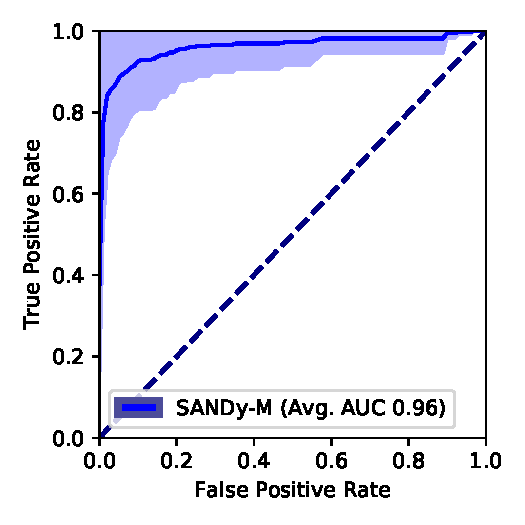
\includegraphics[width=\textwidth]{diagrams/roc_with_uncertainty_stationary.pdf}
  \caption{\textsc{StationaryMP}}
  \end{subfigure}%
\hfill
\begin{subfigure}{.3\textwidth}
  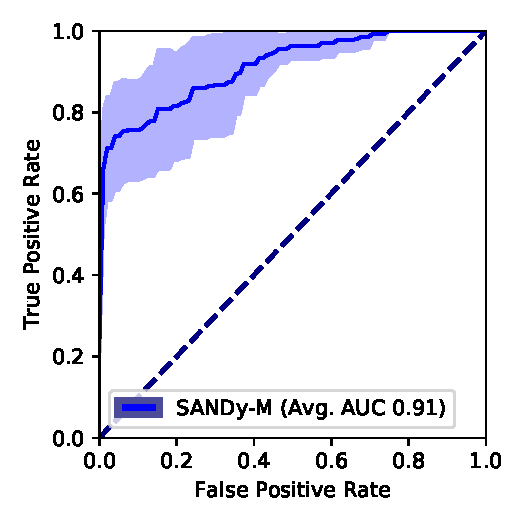
\includegraphics[width=\textwidth]{diagrams/roc_with_uncertainty_nonstationary.pdf}
  \caption{\textsc{$\epsilon$-NonstationaryMP}}
  \end{subfigure}%
\hfill
\begin{subfigure}{.3\textwidth}
  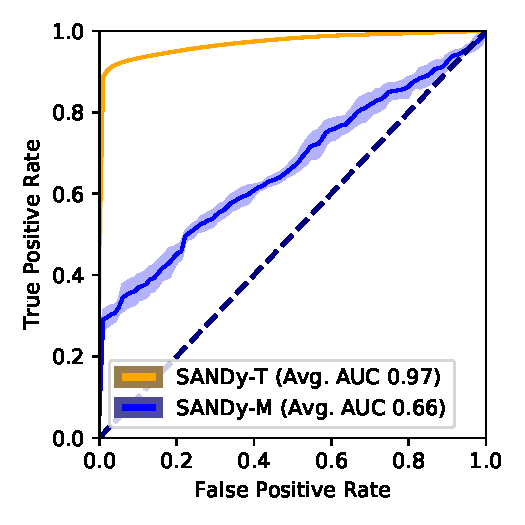
\includegraphics[width=\textwidth]{diagrams/roc_with_uncertainty_spriteworld.pdf}
  \caption{\texttt{Spriteworld}}
\end{subfigure}%
\caption{ 
ROC plots for correct sparsity patter prediction on the three environments.
On held-out test transitions we derive the ground truth local connectivity per step---label information that is \emph{not} used to train the attention model---and measure (over 5 runs; $1$ std. dev. shaded) true and false positive rates while sweeping the mask threshold $\tau$ over its allowable range.
An accurate model generates an Area Under the Curve (AUC) close to $1$.
We observe that while SANDy-Mixture is sufficient for (nearly) solving the simpler synthetic MP environments, it underperforms in Spriteworld.
SANDy-Transfomer, which has a stronger inductive bias, is sufficient to (nearly) solve Spriteworld.
}
\label{fig:roc}
\end{figure}

Figure \ref{fig:roc} shows that while the SANDy-Mixture is sufficient to solve the simpler synthetic MP settings (with avg AUC of $0.96$ and $0.91$ for the stationary and non-stationary variants), it scales poorly to the Spriteworld environment.
While the modest inductive bias of sparse local connections and high-entropy mixture components in SANDy-Mixture makes it widely applicable, we hypothesize that its sensitivity to hyperparameters makes it difficult to tune in complex settings.
Fortunately, SANDy-Transformer, performs favorably in Spriteworld by incorporating a stronger inductive bias about the state subspace structure.
Thus we use SANDy-Transformer to perform local factorization inference in the remaining experiments.


\begin{figure}[ht]
\centering
\subcaptionbox{SANDy-Mixture}{
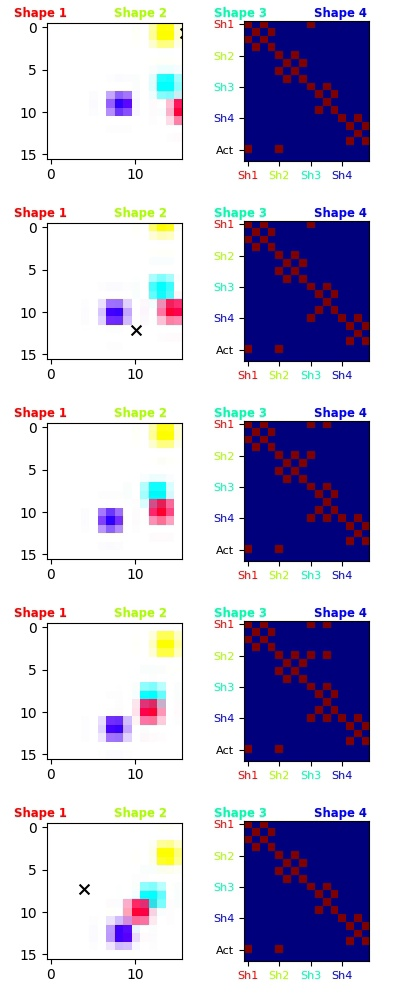
\includegraphics[width=0.4\textwidth]{diagrams/selected_frames_mmn.jpg}
\label{fig:qual_attn_left}
}
\subcaptionbox{SANDy-Transformer}{
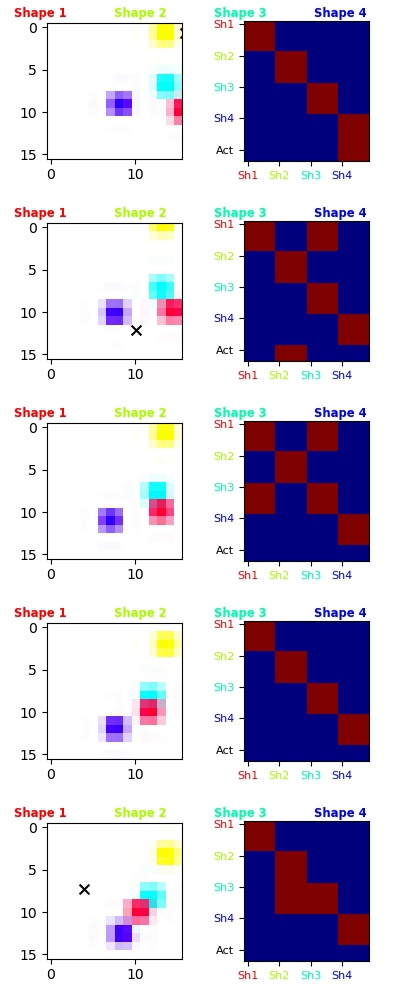
\includegraphics[width=0.4\textwidth]{diagrams/selected_frames_ssa.jpg}
\label{fig:qual_attn_right}
}
\caption{
Qualitative comparison of two attention mechanisms on the same \texttt{Spriteworld} trajectory.
\textbf{SANDy-Mixture} (left) has a weaker inductive bias as it relies on sparsity regularization alone.
Accordingly, it can learn a more compact subspace (e.g. grid patterns within a shape indicate that $x$ and $y$ coordinates move independently), but is less reliable in attending to collisions between shapes, and completely fails to attend to the action's affect on shapes.
\textbf{SANDy-Transformer} has a stronger inductive bias and can more reliably infer the local interaction pattern between the five subspaces (four shapes and one action).
}
\label{fig:qual_attn}
\end{figure}

Figure \ref{fig:qual_attn} provides some qualitative intuition as to how the two variants of SANDy differ in their attention strategy in the Spriteworld environment.

\section{Fitting dynamics models to Spriteworld}\label{appdx_dynamics_modeling}

\begin{figure}[!t]
\centering
\subcaptionbox{Ground Truth}{
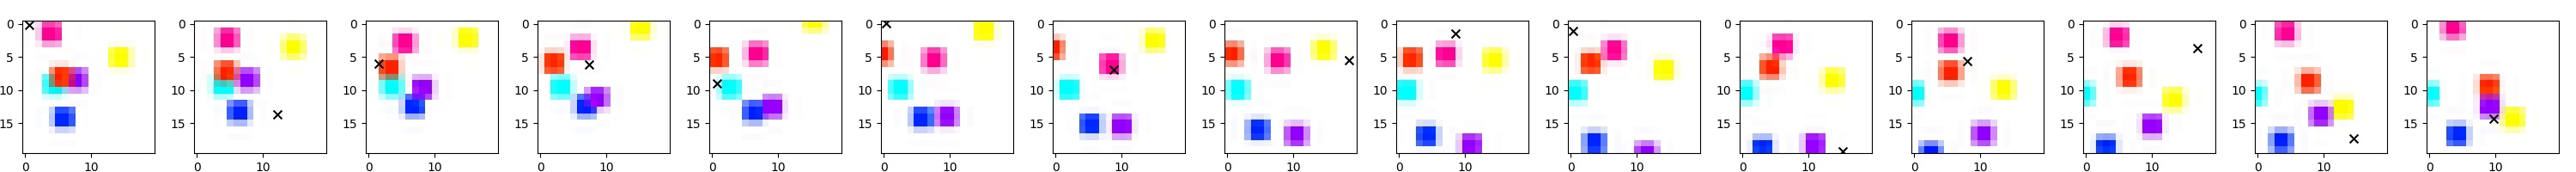
\includegraphics[width=1.0\textwidth]{diagrams/selected_frames_GroundTruth.jpg}
\label{fig:qual_dynamics_models_1}
}
\subcaptionbox{Linear Dynamics}{
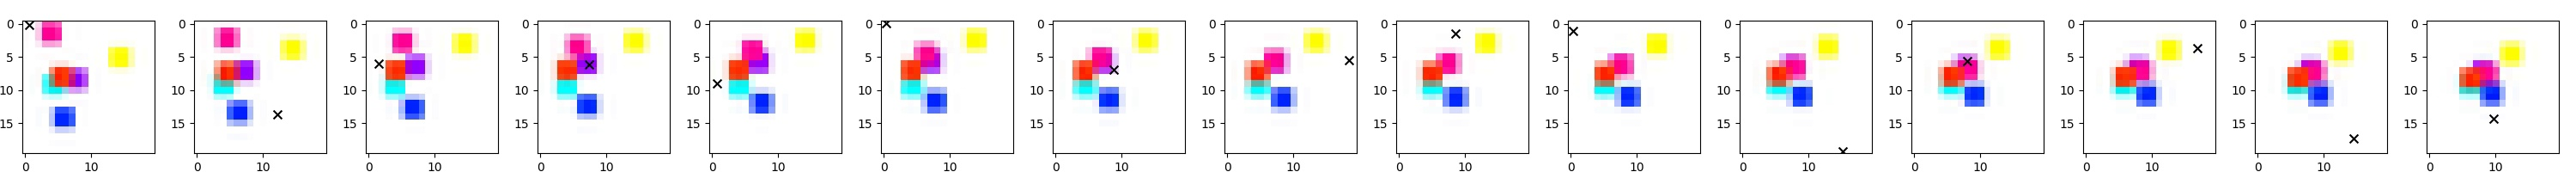
\includegraphics[width=1.0\textwidth]{diagrams/selected_frames_Linear.jpg}
\label{fig:qual_dynamics_models_2}
}
\subcaptionbox{MLP Dynamics}{
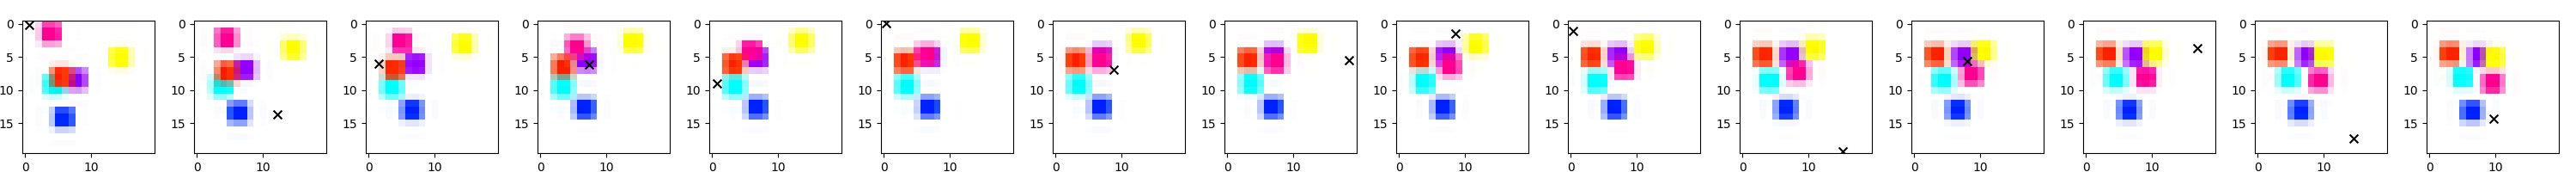
\includegraphics[width=1.0\textwidth]{diagrams/selected_frames_MLP.jpg}
\label{fig:qual_dynamics_models_3}
}
\subcaptionbox{LSTM Dynamics}{
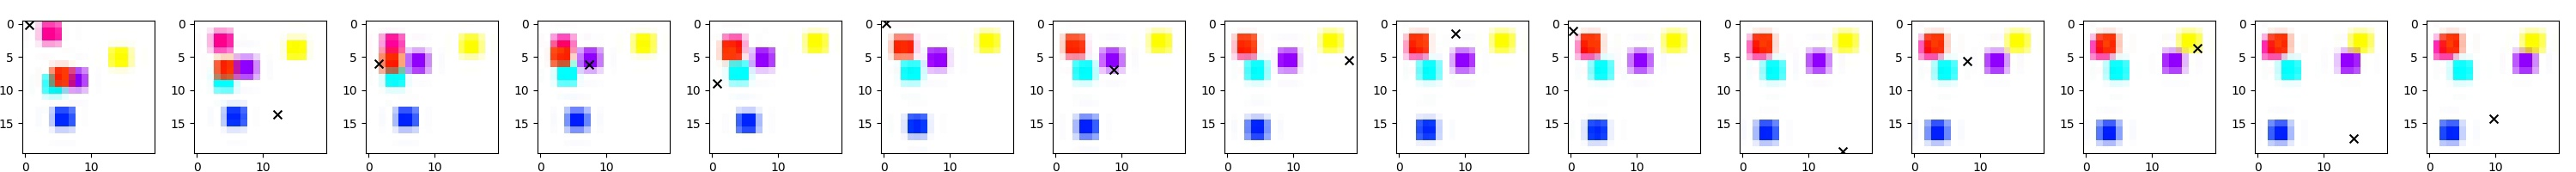
\includegraphics[width=1.0\textwidth]{diagrams/selected_frames_LSTM.jpg}
\label{fig:qual_dynamics_models_4}
}
\caption{
Auto-regressive model-based rollouts for a variety of dynamics models fit to Spriteworld.
While the dynamics models were able to achieve relatively low error in the next-state prediction task, they fail to capture collisions and long-term dependencies in the sampled trajectories, and thus were omitted as baselines in the RL experiments.
All trajectories share the same initial state.
}
\label{fig:qual_dynamics_models}
\end{figure}

Since CoDA is a data augmentation strategy, it is reasonable to consider an alternative approach to augmenting the experience buffer: sampling from a dynamics model as in model-based RL.
Here we present some qualitative results from our efforts in fitting dynamics models to the Spriteworld environment.
We found that while dynamics models achieve a decent error in the next-state prediction task, they fail to produce a diverse set of trajectories when used as autoregressive samplers.
In particular, the autoregressive sampling did not model collisions well and often produced trajectories where sprites converged to fixed points in space after a short number of steps.
Figure \ref{fig:qual_dynamics_models} shows trajectories sampled autoregressively from Linear, MLP, and LSTM-based dynamics models, alongside the ground truth trajectory.
Note that all dynamics models were trained to minimize error in next-state prediction given the current state and action. 
In other words the LSTM auto-regressively predicts successive dimensions of the next state rather than modeling multiple time steps of the trajectory.
Nevertheless the environment is truly Markov because instantaneous velocities are observed, so this information should be sufficient in theory to capture the environment dynamics.

\section{Sample efficient dynamics modeling with CoDA}\label{appdx_coda_for_mbrl}

\begin{figure}[h!]
\centering
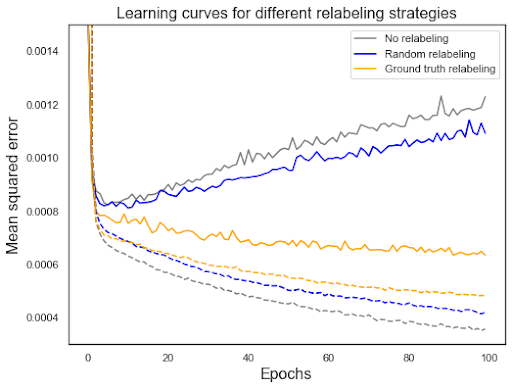
\includegraphics[width=0.5\textwidth]{diagrams/modelbased_training_plot.png}
\caption{
Learning curves for training a forward dynamics model using data from a random policy. Dotted lines indicate training performance, whereas solid lines indicate validation performance. We see that using the ground truth mask prevents overfitting and allows us to achieve much better validation performance. 
}
\label{fig:training_forward_model}
\end{figure}

If we had access to the ground truth local factorization, even for a few samples (e.g., we could have humans label them), how much more efficient would it be to train a dynamics model? In Figure \ref{fig:training_forward_model}, we sample 2000 transitions from a random policy in Spriteworld and use the data to train a forward dynamics model using MSE loss. The validation loss throughout training is plotted. Our baseline uses only the initial dataset, and quickly overfits the training set, showing increasing error after the initial few epochs. The same applies to a ``random'' CoDA strategy, that does CoDA using an identity attention mask ($M(s, a) = I \ \forall \ (s, a)$) to randomly relabel the components. The random strategy does a bit better than the no CoDA strategy, since the randomness acts as a regularizer. Finally, we train a model using an additional 35,000 unique counterfactual CoDA transitions, and find that it significantly improves validation loss and prevents the model from overfitting. Note that we could have generated many more CoDA samples: from 2000 base transitions, if 80\% of them do not involve collisions and there are 4 connected components in each, we could generate as many as $1600^4$ (6.5 trillion!) counterfactual samples.  

\section{Compute Infrastructure}

Experiments were run on a mix of local machines and a compute cluster, with a mix of GTX 1080 Ti, Titan XP, and Tesla P100 GPUs. This was solely to run jobs in parallel, and all experiments can be run locally (GPU optional for \texttt{Spriteworld} and \texttt{Pong}, but recommended for \texttt{Fetch} experiments).

\end{document}